\chapter[Revisione]{Come approvare i contenuti prodotti dagli utenti}

%\begin{landscape}
\begin{figure}[H]
 \centering
 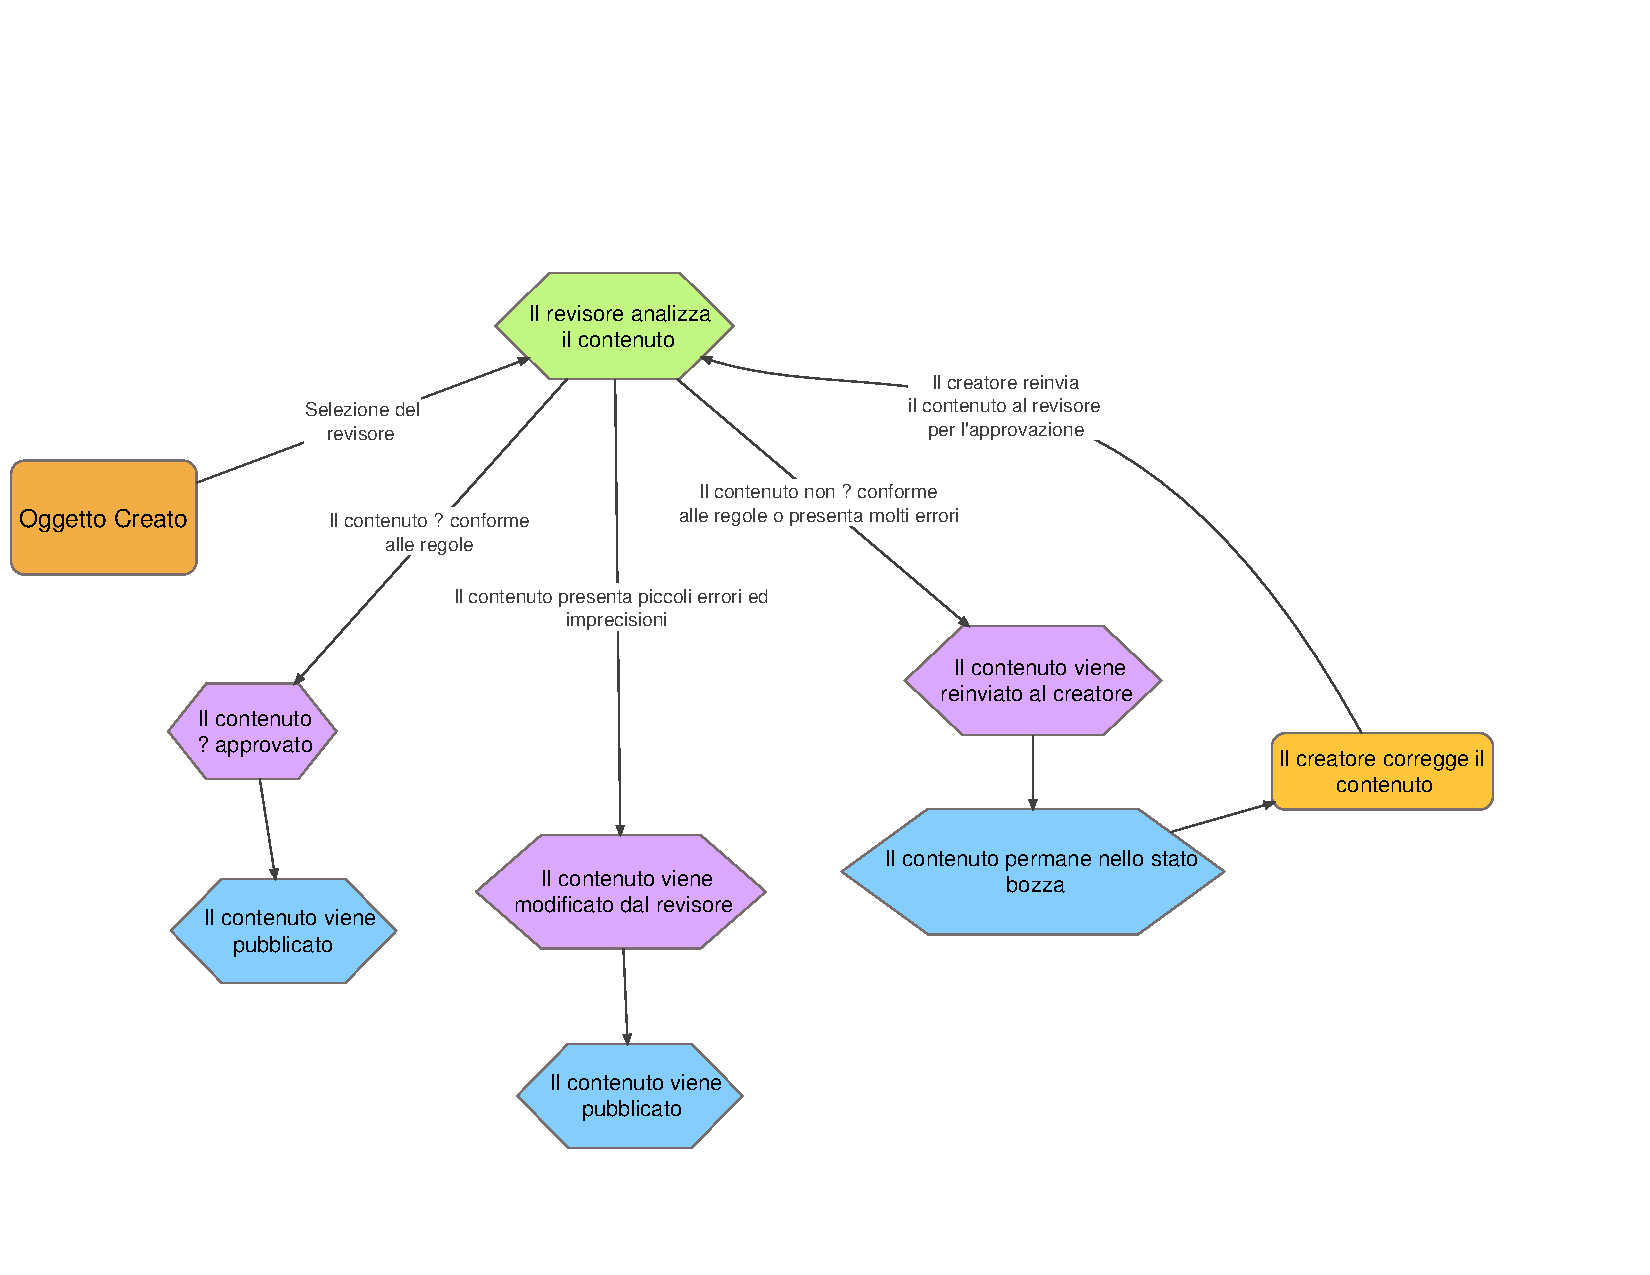
\includegraphics[width=\textwidth]{./immagini/chapter_approval/revisione.pdf}
 % approve_workflow1.png: 928x176 pixel, 72dpi, 32.74x6.21 cm, bb=
 \caption{Flusso per l'approvazione di un contenuto}
 \label{fig:approve_workflow1}
\end{figure}
%\end{landscape}

\section{Esempio di approvazione}

Il cms scolastico  mette a disposizione degli editori un sistema per la revisione dei contenuti prima che questi siano approvati. Un piccolo esempio ci permetterà di capire come funziona il sistema per la revisione. Immagineremo che uno studente \textsl{Gianni} sia stato incaricato da un suo insegnante \textsl{Prof. Matematica} di creare un articolo all'interno dello spazio riservato alla sua clase.
Gianni crea quindi un articolo nello spazio riservato alla 5B e lo pubblica. Siccome Gianni è un utente  i cui permessi non sono sufficienti per la pubblicazione immediata viene inviato alla pagina di selezione dei revisori fig.\ref{fig:approve_select1}
\begin{figure}[H]
 \centering
 \includegraphics[width=\textwidth]{./immagini/chapter_approval/approve_select1.png}
 % approve_select1.png: 1264x249 pixel, 72dpi, 44.59x8.78 cm, bb=
 \label{fig:approve_select1}
\end{figure}
Cliccando su aggiungi utenti Gianni potrà selezionare il Prof. di Matematica, quando Gianni sottoporrà a revisione altri articoli tutti i revisori precedenti saranno ricordati in modo da permettere un più celere processo di approvazione fig.\ref{fig:approve_select10}
\begin{figure}[H]
 \centering
 \includegraphics[width=\textwidth]{./immagini/chapter_approval/approve_select10.png}
 % approve_select1.png: 1264x249 pixel, 72dpi, 44.59x8.78 cm, bb=
\caption{Durante un successivo processo di approvazione i precedenti revisori sono automaticamente resi disponibili} 
\label{fig:approve_select10}
\end{figure}

\begin{figure}[H]
 \centering
 \includegraphics[width=\textwidth]{./immagini/chapter_approval/approve_select2.png}
 % approve_select1.png: 1264x249 pixel, 72dpi, 44.59x8.78 cm, bb=
\caption{Gianni selezione il revisore scorrendo la lista degli utenti}  
\label{fig:approve_select2}
\end{figure}

Dopo aver selezionato il revisore e continuato il flusso di lavoro Gianni può inviare un messaggio al suo revisore circa possibili problemi che quest ultimo potrebbe incontrare.
\begin{figure}[H]
 \centering
 \includegraphics[width=\textwidth]{./immagini/chapter_approval/approve_select3.png}
 % approve_select1.png: 1264x249 pixel, 72dpi, 44.59x8.78 cm, bb=
\caption{Dopo aver selezionato il revisore questo compare nella lista degli utenti revisori del contenuto appena pubblicato}
\label{fig:approve_select3}
\end{figure}

Il messaggio sarà reso disponibile all'utente revisore che potrà comunicare con Gianni attraverso l'interfaccia di approvazione.

\begin{figure}[H]
 \centering
 \includegraphics[width=\textwidth]{./immagini/chapter_approval/approve_select4.png}
 % approve_select1.png: 1264x249 pixel, 72dpi, 44.59x8.78 cm, bb=
\caption{Gianni può mandare un messaggio all'utente revisore}
\label{fig:approve_select4}
\end{figure}

Gianni potrà monitorare lo stato dei suoi articoli nella sua area riservata (\textsl{Il mio profilo}) 

\begin{figure}[H]
 \centering
 \includegraphics[width=\textwidth]{./immagini/chapter_approval/approve_select5.png}
 % approve_select1.png: 1264x249 pixel, 72dpi, 44.59x8.78 cm, bb=
\caption{Stato dell'articolo appena pubblicato} 
\label{fig:approve_select5}
\end{figure}

\begin{figure}[H]
 \centering
 \includegraphics[width=\textwidth]{./immagini/chapter_approval/approve_select6.png}
 % approve_select1.png: 1264x249 pixel, 72dpi, 44.59x8.78 cm, bb=
\caption{L'articolo appena creato da Gianni attende di essere approvato o respinto} 
\label{fig:approve_select6}
\end{figure}

L'utente revisore, in questo caso il Prof. di Matematica riceve nella sua area personale (e via e-mail) un avviso circa il nuovo contenuto in attesa di approvazione. Il Prof. di Matematica entra nella sua area personale e dal menu \textsl{Collaborazione} vede il contenuto creato da Gianni:

\begin{figure}[H]
 \centering
 \includegraphics[width=\textwidth]{./immagini/chapter_approval/approve_select7.png}
 % approve_select1.png: 1264x249 pixel, 72dpi, 44.59x8.78 cm, bb=
 \label{fig:approve_select7}
\end{figure}

Cliccando sulla voce nel menu Collaborazione il Prof. può vedere un'anteprima del lavoro di Gianni e decidere se:
\begin{itemize}
 \item Approvare il contenuto
\item Modificare il contenuto ed approvarlo
\item Rimandare il contenuto a Gianni affinchè questo lo modifichi
\end{itemize}
\begin{figure}[H]
 \centering
 \includegraphics[width=\textwidth]{./immagini/chapter_approval/approve_select8.png}
 % approve_select1.png: 1264x249 pixel, 72dpi, 44.59x8.78 cm, bb=
 \label{fig:approve_select8}
\end{figure}

Se il contenuto è stato approvato  dopo circa 5 minuti sarà disponibile nella zona pubblica del sito.
\begin{figure}[H]
 \centering
 \includegraphics[width=\textwidth]{./immagini/chapter_approval/approve_select9.png}
 % approve_select1.png: 1264x249 pixel, 72dpi, 44.59x8.78 cm, bb=
\caption{Il sistema notifica la avvenuta approvazione del contenuto} 
\label{fig:approve_select9}
\end{figure}

\section{Creazione del Workflow}

Per abilitare il sistema di approvazione è necessario creare dal backend amministrativo un workflow, ovvero un insieme di azioni da intraprendere sul contenuto quando una determinata condizione è soddisfatta. Dal menu impostazioni scegliamo Workflow ed entramo nella collezione standard di workflow:
\begin{figure}[H]
 \centering
 \includegraphics[width=\textwidth]{./immagini/chapter_approval/approve_workflow1.png}
 % approve_workflow1.png: 928x176 pixel, 72dpi, 32.74x6.21 cm, bb=
 \caption{Per abilitare l'approvazione dei contenuti è necessario creare un oggetto all'interno della catena dei flussi di lavoro}
 \label{fig:approve_workflow2}
\end{figure}
Creiamo quindi un workflow che verrà eseguito ogni volta che un utente di un particolare gruppo pubblica un contenuto:

\begin{figure}[H]
 \centering
 \includegraphics[width=\textwidth]{./immagini/chapter_approval/approve_workflow_create.png}
 % approve_workflow_create.png: 930x350 pixel, 72dpi, 32.81x12.35 cm, bb=
 \caption{Una volta selezionato il gruppo di workflow di interesse dobbiamo creare un nuovo workflow}
 \label{fig:approve_create}
\end{figure}
Per il workflow di approvazione descritto nell'esempio precedente selezioniamo l'evento Revisione Avanzata:

\begin{figure}[H]
 \centering
 \includegraphics[width=\textwidth]{./immagini/chapter_approval/approve_workflow_creation.png}
 % approve_workflow_creation.png: 928x265 pixel, 72dpi, 32.74x9.35 cm, bb=
 \caption{Durante la creazione del workflow per l'approvazione dobbiamo selezionare quali eventi intendiamo inserire}
 \label{fig:approve_create1}
\end{figure}

Nel interfaccia di modifica/creazione ci viene chiesto di inserire alcuni parametri:
\begin{figure}[H]
 \centering
 \includegraphics[width=\textwidth]{./immagini/chapter_approval/approve_workflow_edit1.png}
 % approve_workflow_edit1.png: 924x564 pixel, 72dpi, 32.60x19.90 cm, bb=
 \caption{L'evento revisione avanzata mette a disposizione due modalità: approvazione con revisori preselezionati e approvazione con revisori selezionati dagli utenti}
 \label{fig:approve_edit1}
\end{figure}

\begin{description}
 \item[Sezioni interessate] Le sezioni del sito soggette ad approvazione, nell'esempio la sezione Alunni
\item[Sistema di revisione]È possibile scegliere tra una lista predefinita di Revisori oppure lasciare la scelta all'utente come nell'esempio
\item[Gruppi di utenti esclusi]Gli utenti appartenenti a questi gruppi possono sempre pubblicare istantaneamente i contenuti
\end{description}



\begin{figure}[H]
 \centering
 \includegraphics[width=\textwidth]{./immagini/chapter_approval/approve_workflow_edit2.png}
 % approve_workflow_edit2.png: 928x544 pixel, 72dpi, 32.74x19.19 cm, bb=
 \label{fig:approve_edit2}
\end{figure}

Dopo aver creato e salvato il workflow dobbiamo associarlo ad un trigger tramite il menu Impostazioni->Triggers. Nel nostro caso il workflow dovrà essere associato al trigger content::publish::before
\begin{figure}[H]
 \centering
 \includegraphics[width=\textwidth,bb=0 0 929 450]{./immagini/chapter_approval/approve_trigger1.png}
 % approve_trigger1.png: 929x450 pixel, 72dpi, 32.77x15.88 cm, bb=0 0 929 450
 \caption{Dopo aver creato il workflow è necessario associarlo ad un opportuno trigger}
 \label{fig:approve_trigger1}
\end{figure}
\begin{figure}[H]
 \centering
 \includegraphics[width=\textwidth]{./immagini/chapter_approval/approve_trigger2.png}
 % approve_trigger2.png: 928x95 pixel, 72dpi, 32.74x3.35 cm, bb=
 \label{fig:approver_trigger2}
\end{figure}









